% Problem 1 - CS amplifier transfer characteristic (18 points)
\Point{cstransfer}{findpointsab}{4}
\Point{cstransfer}{biaspoint}{3}
\Point{cstransfer}{maxamplitude}{3}
\Point{cstransfer}{gainandtransconductance}{4}
\Point{cstransfer}{lambdaeffect}{4}
\begin{mainquestion}{cstransfer}{Common Source Amplifier Transfer Characteristic}

Consider a common source (CS) amplifier as shown below. The key parameters are $V_{DD} = 10\ \text{V}$, $R_{D} = 3.4\ \text{k}\Omega$, $k_{n} = k_{n}^{\prime}\frac{W}{L} = 10\ \frac{\text{mA}}{V^{2}}$, and $V_{t} = 0.7\ \text{V}$. Assume $\lambda = 0$ for parts (a)-(d).

\begin{center}
\includegraphics[width=2in]{../v0/Picture1.png}
\quad
\includegraphics[width=3in]{../v0/Picture2.png}
\end{center}

\begin{partquestion}{findpointsab}{Find the coordinates of points A and B (i.e., $V_{I}$ and $V_{O}$) on the sketch in figure (b) above.}
\begin{answer}
\begin{kaitlyn}

\noindent\fbox{%
    \begin{minipage}{\dimexpr\textwidth-2\fboxsep-2\fboxrule\relax}
        \textbf{Why we're doing this problem:} Points A and B define the boundaries of the amplifier’s useful operating region, where the output looks like a scaled version of the input -- which is what we want: given some input signal, predict what signal comes out!
    \end{minipage}%
}



\end{kaitlyn}
Point A on the sketch corresponds to the moment when the transistor transitions from cut-off to saturation. This occurs when $v_{I} = v_{GS} = V_{t} = 0.7\ \text{V}$. At this point, current is just beginning to flow so $v_{DS} = v_{O} = V_{DD}$. So, point A is (0.7 V, 10 V).

Point B corresponds to the moment where the transistor goes from saturation to triode. In this case, $V_{DS} = V_{GS} - V_{t}$ so $v_{O} = v_{I} - V_{t} = v_{I} - 0.7\ \text{V}$. Because at point B we are at the boundary of two regions, either formula for $I_{D}$ should work (also because $\lambda = 0$, which ensures continuity between regions with our standard formulas for $I_{D}$). Choosing that of saturation gives:

\[
I_{D} = \frac{V_{DD} - v_{O}}{R_{D}} = \frac{1}{2} k \left(V_{GS} - V_{t}\right)^{2}
\]

so

\[
\frac{10 - v_{O}}{3.4} = \frac{1}{2}(10)(v_{I} - 0.7)^{2} = \frac{1}{2}(10)v_{O}^{2}
\]

this leads to the quadratic:

\[
5 v_{O}^{2} + 0.2941 v_{O} - 2.9412 = 0
\]

which has solutions $v_{O} = -0.797$ and $v_{O} = 0.738$. Only the second is a valid solution. From here, $v_{I} = v_{O} + 0.7 = 1.438\ \text{V}$, so point B is (1.438 V, 0.738 V).

\begin{kaitlyn}

\textbf{Zooming out:} We’re moving one level higher in abstraction: zooming out from the MOSFET as an individual device to the MOSFET as an amplifier. The same $V_{GS}$, $V_{DS}$, and $I_{D}$ and region-of-operation tools still apply from previous lectures, but now we use them to understand the circuit-level relationship between $v_O$ and $v_O$. Ultimately, that is what we want from an amplifier: given some input signal, predict what signal comes out. Once we understand this input-output behavior, we can characterize the amplifier by parameters like gain, $R_i$, and $R_o$, and eventually treat the entire amplifier as a building block in a larger circuit.

    
\end{kaitlyn}


    
\end{answer}
\end{partquestion}

\begin{partquestion}{biaspoint}{If the amplifier is biased to operate with an overdrive voltage $V_{OV} = V_{GS} - V_{t} = 0.5\ \text{V}$, find the bias point Q on the transfer characteristic. What is the value of $I_{D}$ when operating at the bias point Q?}
\begin{answer}
We know with this overdrive voltage level:

\[
v_{I} = V_{GS} = V_{OV} + V_{t} = 0.5 + 0.7 = 1.2\ \text{V}.
\]

We can use the same equation as in part (a) to find the output voltage:

\begin{gather*}
    \frac{10 - v_o}{3.4} = \frac{1}{2}(10)(v_I - 0.7)^2 = \frac{1}{2}(10)v_{OV}^2 = 5(0.5)^2 = 1.25 \\
    v_o = 10 - (1.25)(3.4) = \qty{5.75}{\volt}
\end{gather*}

The point Q is therefore (1.2 V, 5.75 V). It follows that:

\[
I_{D} = \frac{10 - v_{O}}{3.4} = \frac{10 - 5.75}{3.4} = \qty{1.25}{\milli\ampere}.
\]
\end{answer}
\end{partquestion}
\begin{partquestion}{maxamplitude}{At the bias point Q, what is the largest amplitude of a sine-wave voltage signal that can be applied at the input while the transistor remains in saturation? What is the peak-to-peak voltage of the output signal that results?}
\begin{answer}

\begin{kaitlyn}

    Beginning with our DC bias point:
    \begin{align*}
        (\qty{1.2}{\volt}, \qty{5.75}{\volt})
    \end{align*}
    
    we need to consider the AC time-varying component 
    \begin{align*}
        v_I(t) = V_{GS} + v_{gs}(t)
    \end{align*}
    

    and how big a signal $v_{gs}$ can be applied before it pushes the transistor out of saturation regime.

    We know that anything beyond our previously-found bounds, point A (\qty{0.7}{\volt}, \qty{10}{\volt}) and point B (\qty{1.438}{\volt}, \qty{0.738}{\volt}), would push the transistor out of saturation. 

    (If it helps, try drawing out a simple sine wave to help visualize, making sure it's offset at \qty{1.2}{\volt}, and seeing which bound you hit first, \qty{1.438}{\volt} or \qty{0.7}{\volt} from \qty{1.2}{\volt}!) 

    
\end{kaitlyn}
Since our quiescent point Q has an input voltage which is closer to point B's input voltage than it is to point A's input voltage, a sine wave centered on point Q (about \qty{1.2}{\volt}) will hit a limiting point at B (\qty{1.438}{\volt}) when its amplitude is $1.438 - 1.2 = \qty{0.238}{\volt}$. 
\begin{kaitlyn}
    \begin{figure}
        \centering
        \includegraphics[width=0.5\linewidth]{sine_swing_limits.png}
        \label{fig:cstransfer:sineswing}
    \end{figure}
\end{kaitlyn}
While there will be distortion due to the square-law relationship of the current in the saturation regime, it will remain in saturation. With an input sine wave of amplitude of \qty{0.238}{\volt}, at the maximum input, the output will dip to \qty{0.738}{\volt} (since we are touching point B). 

At the minimum input, the output will rise to a value determined by an input $v_{I} = 1.2 - 0.238 = \qty{0.962}{\volt}$ as follows:
\begin{align*}
    \frac{10 - v_O}{3.4} &= \frac{1}{2}(10)(v_I - 0.7)^2 \\
    10 - v_O &= (5)(3.4)(0.962 - 0.7)^2 \\
    v_O &= 10 - (5)(3.4)(0.962 - 0.7)^2 \\
    &= \qty{8.83}{\volt}
\end{align*}

The peak-to-peak voltage of the output signal is then $8.83 - 0.738 = \qty{8.095}{\volt}$.


\begin{kaitlyn}
    \noindent\fbox{%
    \begin{minipage}{\dimexpr\textwidth-2\fboxsep-2\fboxrule\relax}
        \textbf{Developing Intuition:} Real signals that go into systems are rarely ever clean DC voltages (ex: a microphone, antenna will produce a voltage that changes with time). Since we know the bounds in which the amplifier circuit will operate in its linear regime (through MOSFET saturation equations), we can then determine how large an AC signal input can be for our specific system. But actually, usually circuit designers work the other way: they are given an AC amplitude spec and they design their system to be able to meet it.
    \end{minipage}%
    }
\end{kaitlyn}

\end{answer}
\end{partquestion}

\begin{partquestion}{gainandtransconductance}{What are the transconductance $g_{m}$ and gain $A_{v}$ at point Q? Provide the gain both in linear (V/V) and log (dB) units.}
\begin{answer}


The transconductance is:

\begin{align*}
    g_m &= k(V_{GS} - V_t) \\
    &= 10(1.2 - 0.7) \\
    &= \qty{5.0}{\milli\siemens}
\end{align*}

The gain (ignoring output resistance) is:

\[
A_{vo} = -g_{m} R_{D} = -5(3.4) = -17\ \frac{\text{V}}{\text{V}}
\]

which, in decibels is:

\[
A_{vo,\text{dB}}= 20\log|A_{vo}| = 20\log|17| = 24.6\ \text{dB}.
\]

\end{answer}
\end{partquestion}

\begin{partquestion}{lambdaeffect}{Now consider the MOSFET has a non-zero channel-length modulation parameter $\lambda$. What is the maximum $\lambda$ allowed so the voltage gain does not fall below 24 dB? What is the minimum output resistance $r_{o}$? (You may assume the bias point Q is not affected by $\lambda$.)  }
\begin{answer}

\begin{kaitlyn}
    \noindent\fbox{%
    \begin{minipage}{\dimexpr\textwidth-2\fboxsep-2\fboxrule\relax}
        \textbf{What we're really answering:} MOSFETs are not ideal. How much MOSFET non-ideality can we tolerate before the entire amplifier fails to meet its required gain?
    \end{minipage}%
    }

    
\end{kaitlyn}

\begin{kaitlyn}


 Until now, we assumed $\lambda=0$, meaning our MOSFET behaved like an ideal current source in saturation. Once $V_{GS}$ set $I_D$, changing $V_{DS}$ did not change the drain current:


 \[\lambda=0 \qquad \Longrightarrow \qquad r_o=\infty.\]

Real MOSFETs are not ideal current sources. Due to \textbf{channel-length modulation}, increasing $V_{DS}$ causes $I_D$ to increase slightly even when the transistor remains in saturation. This is why the saturation-region $I_D$--$V_{DS}$ curves are not perfectly flat.

We capture this non-ideality in the small-signal model with

\[r_o=\frac{1}{\lambda I_D}.\]

A larger $\lambda$ therefore means a smaller $r_o$: the MOSFET behaves less like an ideal current source.


\textbf{Follow the figure on the next page with the small signal model drawn out and how it fits back into the larger circuit!}

\begin{figure}
    \centering
    \includegraphics[width=1\linewidth]{small_signal_ro_notes.jpeg}
    \label{fig:cstransfer:smallsignalnotes}
\end{figure}
$r_o$ belongs to the small-signal model of the MOSFET, but the MOSFET is only one part of our common-source amplifier. When we put its small-signal model back into the complete circuit, $V_{DD}$ becomes AC ground, so both $R_D$ and $r_o$ connect from the output node to ground. Thus, the current $g_m v_{gs}$ sees

\[R_D \parallel r_o,\]

and the amplifier gain becomes

\[A_v=-g_m(R_D\parallel r_o)\]

rather than the ideal result $A_v=-g_mR_D$.
\end{kaitlyn}

With output resistance, the formula for the gain is modified slightly:

\[
A_{vo} = -g_{m} \left(R_{D} \parallel r_{o}\right) = -\frac{g_{m} R_{D} r_{o}}{R_{D} + r_{o}}
\]

Because the minimum gain must be 24 dB, we have:

\begin{align*}
    20\log|A_v| &\geq 24 \\
    20\log\left(\frac{g_m R_D r_o}{R_D + r_o}\right) &\geq 24 \\
    \left(\frac{g_m R_D r_o}{R_D + r_o}\right) &\geq 10^\frac{6}{5} \\
    g_m R_D r_o &\geq 10^\frac{6}{5}R_D + 10^\frac{6}{5}r_o \\
    r_o &\geq \frac{10^\frac{6}{5}R_D}{g_m R_D - 10^\frac{6}{5}} \\
\end{align*}

Since $r_{o} = \frac{1}{\lambda I_{D}}$, we have:

\begin{align*}
    \lambda &= \frac{1}{r_o I_D} \\
    &\leq \frac{g_m R_D - 10^\frac{6}{5}}{10^\frac{6}{5}R_D I_D} \\
    &\leq \frac{(5) (3.4) - 10^\frac{6}{5}}{10^\frac{6}{5}(3.4)(1.25)} \\
    &\leq \qty{0.0171}{\per\volt} \\
\end{align*}

so, it follows that

\[
r_{o} \geq \frac{1}{\lambda_{\max} I_{D}} = \frac{1}{(0.0171)(1.25)} = 46.8\ \text{k}\Omega.
\]

\begin{kaitlyn}
    \noindent\fbox{%
    \begin{minipage}{\dimexpr\textwidth-2\fboxsep-2\fboxrule\relax}
        \textbf{Why we're doing this problem:} This is where it got tricky. We're bridging our individual MOSFET model to a higher-level, larger circuit model, specifically the common-source amplifier circuit. You should be able to generalize small-signal models and derive gain for any new circuit, from ideal CS amplifiers to new configurations with non-idealities.
    \end{minipage}%
    }
\end{kaitlyn}
\end{answer}
\end{partquestion}

\end{mainquestion}


% Problem 2 - CS amplifier design (12 points)
\clearpage
\Point{csdesign}{mingm}{2}
\Point{csdesign}{idanvov}{5}
\Point{csdesign}{wlratio}{3}
\Point{csdesign}{vgsrange}{2}
\begin{mainquestion}{csdesign}{Common Source Amplifier Design}

A CS amplifier must be designed to provide an output signal with 1.0 V amplitude using a load $R_{D} = 82\ \text{k}\Omega$. Note: This is a design problem; please provide lower \& upper bounds for answers to parts (b)-(d).

\begin{partquestion}{mingm}{If a voltage gain $\left|A_{v}\right| \geq 14\ \frac{\text{V}}{\text{V}}$ is desired, what minimum transconductance $g_{m}$ is required? You may use this $g_{m}$ value to answer the parts below.}
\begin{answer}
If $\lambda = 0$, the gain magnitude of a common source amplifier is:

\[
\left|A_{v}\right| = g_{m} R_{D} \geq 14
\]

so

\[
g_{m} \geq \frac{14}{R_{D}} = \frac{14}{82} = 0.171\ \text{mS}.
\]
\end{answer}
\end{partquestion}

\begin{partquestion}{idanvov}{Using a DC supply $V_{DD} = 3.3\ \text{V}$, what values of $I_{D}$ and $V_{OV} = V_{GS} - V_{t}$ would you choose?}
\begin{answer}
\begin{kaitlyn}

\noindent\fbox{%
\begin{minipage}{\dimexpr\textwidth-2\fboxsep-2\fboxrule\relax}
        \textbf{What this question is asking:} Design a bias point where the resulting output voltage's AC component has enough headroom to swing upwards without hitting the DC rail and  swing downwards without leaving the saturation regime.
\end{minipage}%
}%

Recall our saturation condition:

\[\boxed{V_{DS} \geq V_{OV}}\]

At the DC operating point, the drain voltage is

\[V_{DS,Q} = V_{DD} - I_D R_D.\]

However, $V_{DS}$ changes when an AC input signal is applied. Since the common-source amplifier has negative gain,

\[A_v = -g_mR_D,\]

the worst case for remaining in saturation occurs when the input is at its maximum positive excursion $(+v_{gs})$. At this instant:

\begin{itemize}
    \item the output swings downward, so the drain source voltage becomes $V_{DS,Q}-v_{ds}$, and
    \item the gate-source voltage increases, so the instantaneous overdrive becomes $V_{OV}+v_{gs}$.

\end{itemize}

Therefore, at the worst-case point in the signal swing, we require

\[\boxed{V_{DD} - I_D R_D - v_{ds}\geq V_{OV} + v_{gs} }\]

Notice that this equation contains quantities from both the DC bias point and the AC small-signal model. We now move between these levels of abstraction to rewrite the constraint in terms of $V_{OV}$.

From the MOSFET bias relationship,

\[ g_m = \frac{2I_D}{V_{OV}} \qquad\Rightarrow\qquad I_D = \frac{1}{2}g_mV_{OV}.\]

From the amplifier gain,

\[ |A_v| = \frac{|v_{ds}|}{|v_{gs}|} \qquad\Rightarrow\qquad v_{gs} = \frac{v_{ds}}{|A_v|}.\]

Substituting these relationships into the saturation constraint gives
\end{kaitlyn}

\begin{align*}
V_{DD} - \frac{1}{2}g_{m}V_{OV}R_{D} - v_{ds} &\geq V_{OV} + \frac{v_{ds}}{A_{v}} \\
V_{DD} - v_{ds} - \frac{v_{ds}}{A_{v}} &\geq V_{OV}\left(1 + \frac{1}{2}g_{m}R_{D}\right) \\
V_{OV} &\leq \frac{V_{DD} - v_{ds} - \frac{v_{ds}}{A_{v}}}{1 + \frac{1}{2}g_{m}R_{D}}\\
V_{OV} &\leq \frac{3.3 - 1.0 - \frac{1.0}{14}}{1 + \frac{1}{2}(0.171)(82)}\\
V_{OV} &\leq 0.279\ \text{V}
\end{align*}

and

\begin{align*}
    I_D &= \frac{1}{2} g_m V_{OV} \leq \frac{1}{2} g_m (0.279) \\
    &\leq \frac{1}{2} (0.171)(0.279) \\
    &\leq \qty{0.0238}{\milli\ampere} \\
\end{align*}

At the high end, we can't be too close to the rail in order to allow the small signal output to vary across its maximum amplitude. $V_{DS} \leq V_{DD} - v_{ds} = 3.3 - 1.0 = 2.3\ \text{V}$. The constraints on the current becomes:

\[
I_{D} \geq \frac{V_{DD} - V_{DS}}{R_{D}} = \frac{3.3 - 2.3}{82} = 0.0122\ \text{mA}
\]

and

\[
V_{OV} = \frac{2I_{D}}{g_{m}} \geq \frac{2(0.0122)}{0.171} = 0.143\ \text{V}.
\]

Putting all this together gives the acceptable current range of $12\ \mu\text{A} \leq I_{D} \leq 24\ \mu\text{A}$ and acceptable overdrive voltage range of $0.143\ \text{V} \leq V_{OV} \leq 0.279\ \text{V}$.
\end{answer}
\end{partquestion}

\begin{partquestion}{wlratio}{What $\frac{W}{L}$ ratio is required if $k^{\prime} = \mu_{n} C_{ox} = 70\ \frac{\mu\text{A}}{V^{2}}$?}
\begin{answer}
Since $g_{m} = k'\frac{W}{L}V_{OV}$,

\[
\frac{W}{L} = \frac{g_{m}}{k^{\prime} V_{OV}} = \frac{0.171}{(0.070)V_{OV}} = \frac{2.44}{V_{OV}}
\]

Given the range of $V_{OV}$ from part (\cref{prob:csdesign:idanvov}), we can see the corresponding range for $\frac{W}{L}$: $8.76 \leq \frac{W}{L} \leq 17.08$.
\end{answer}
\end{partquestion}

\begin{partquestion}{vgsrange}{If $V_{t} = 0.6\ \text{V}$, find the range of $V_{GS}$.}
\begin{answer}
Since $V_{GS} = V_{OV} + V_{t} = V_{OV} + 0.6$, we can use the range of $V_{OV}$ from part (\cref{prob:csdesign:idanvov}) to find $0.743\ \text{V} \leq V_{GS} \leq 0.879\ \text{V}$.
\end{answer}
\end{partquestion}

\end{mainquestion}


% Problem 3 - CS amplifier with coupling and distortion (12 points)
\clearpage
\Point{cscoupling}{gainexpression}{3}
\Point{cscoupling}{distortionlimit}{3}
\Point{cscoupling}{currentchange}{3}
\Point{cscoupling}{17dbgain}{3}
\begin{mainquestion}{cscoupling}{Common Source Amplifier with Coupling Capacitors}

A more realistic CS amplifier features coupling capacitors $C_{C1}$ and $C_{C2}$ which are ``large,'' placed there to act as shorts at the small-signal frequencies of interest, without disturbing the DC bias current and voltage. The power supply is set to $V_{DD} = 12\ \text{V}$.

\begin{center}
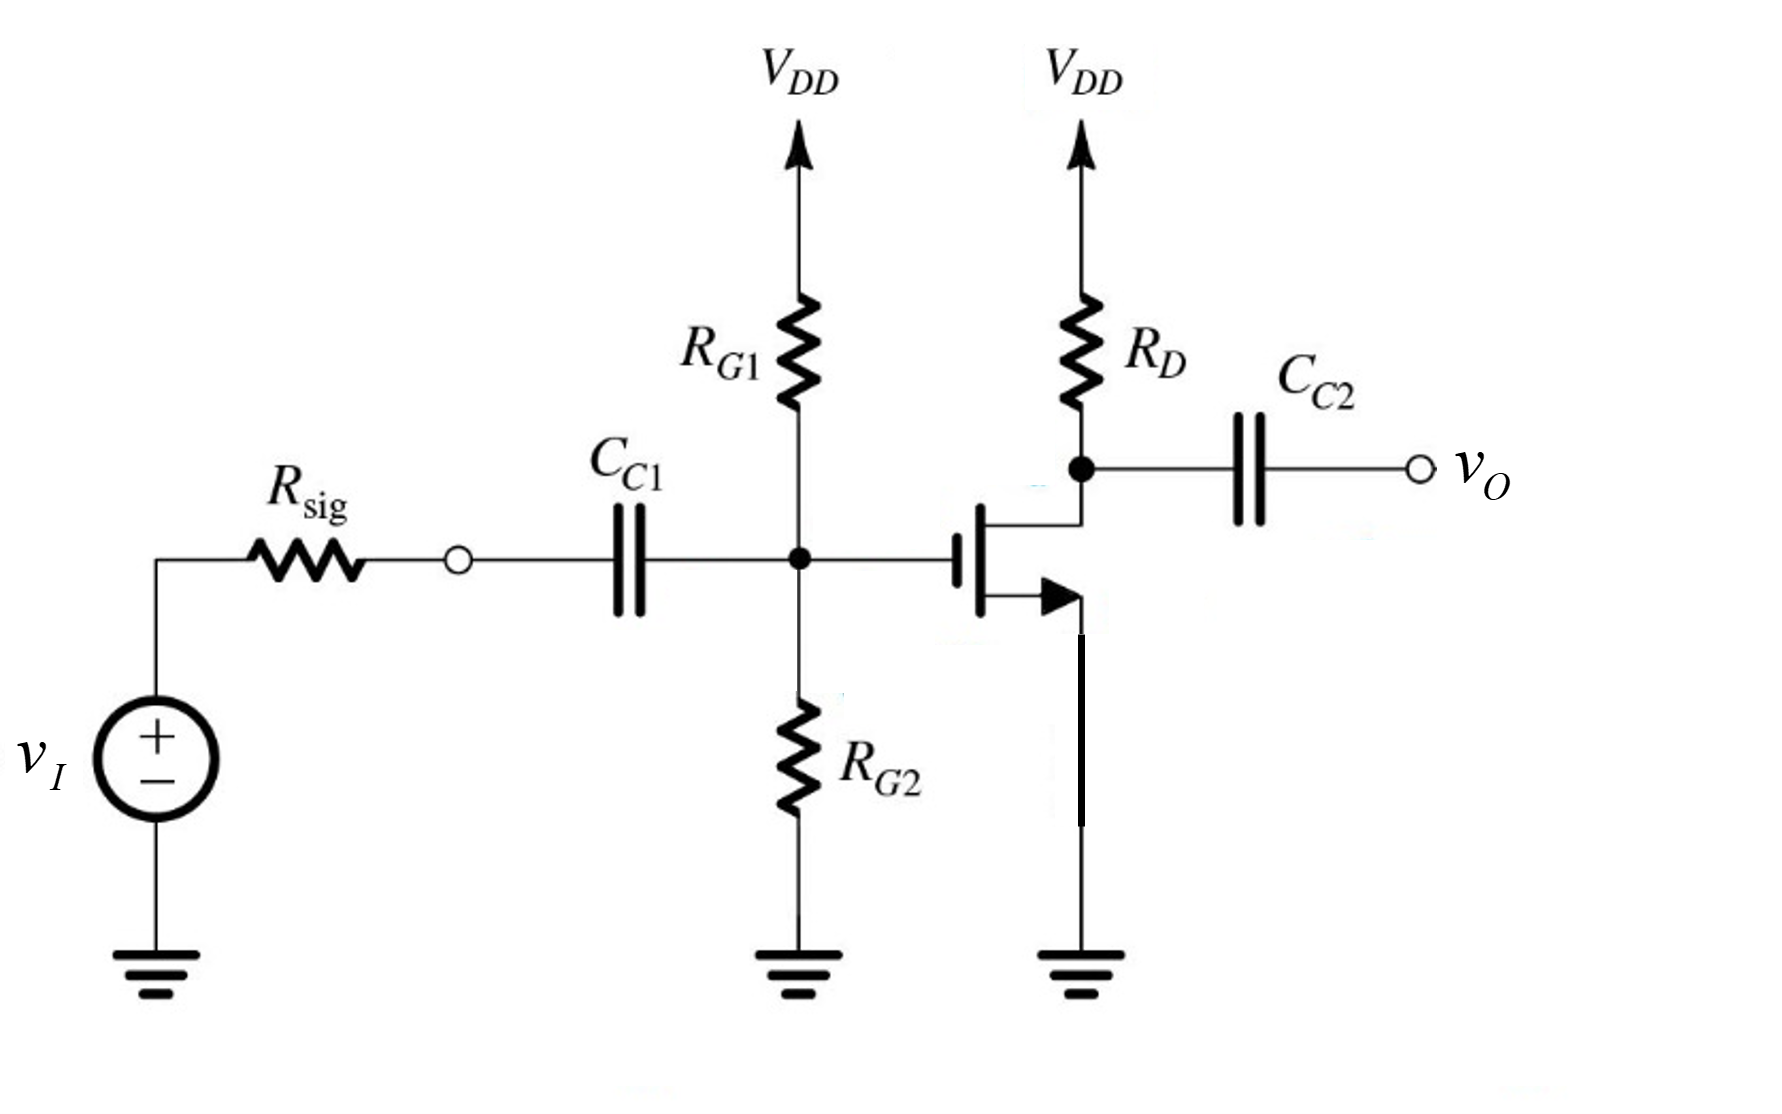
\includegraphics[width=4in]{questionbank/amplifiers/cs_coupling_distortion/v0/schematic.png}
\end{center}

\begin{partquestion}{gainexpression}{The transistor is first biased such that $\frac{1}{3}V_{DD}$ drops across the resistor $R_{D}$. Give a simple expression for the small-signal voltage gain from gate to drain ($A_{v} = \frac{v_{d}}{v_{g}}$) only as a function of $V_{OV} = V_{GS} - V_{t}$. If $V_{OV} \geq 0.4\ \text{V}$, what is the maximum small-signal gain from gate to drain?}
\begin{answer}
Since one-third of the supply voltage $V_{DD}$ drops across the resistor $R_{D}$, we have:

\[
I_{D} = \frac{\frac{V_{DD}}{3}}{R_{D}} = \frac{4}{R_{D}}
\]

The common source gain with $\lambda = 0$ is:

\[
A_{v} = -g_{m}R_{D} = -\frac{2I_{D}}{V_{OV}}R_{D} = -\frac{2(4)}{V_{OV}R_{D}}R_{D} = -\frac{8}{V_{OV}}
\]

For $V_{OV} \geq 0.4$, we have:

\[
\left|A_{v}\right| \leq \frac{8}{0.4} = 20
\]
\end{answer}
\end{partquestion}

\begin{partquestion}{distortionlimit}{With $V_{OV} = 0.4\ \text{V}$, what is the limit to the ``small signal'' amplitude at the gate if we accept a second-order distortion term that is no more than 4\% of the first-order linear term (note this is stricter than the 10\% tolerance we discussed in class)?}
\begin{answer}
We saw from the lecture that the second-order (distortion) term is $\frac{1}{2}k v_{gs}^{2}$, and the first-order (linear) term is $g_{m}v_{gs} = kV_{OV}v_{gs}$. Comparing these two, if we want the second-order term to be less than 0.04 times the first-order term, we have:

\begin{align*}
    \frac{1}{2}k v_{gs}^2 &\leq 0.04 (k V_{OV} v_{gs}) \\
    v_{gs} &\leq 0.08 V_{OV} \\
    v_{gs} &\leq 0.08 (0.4) \\
    v_{gs} &\leq \qty{0.032}{\volt} \\
\end{align*}
\end{answer}
\end{partquestion}

\begin{partquestion}{currentchange}{With the small-signal limits in (b), what is the maximum \% change in $i_{D}$ (relative to $I_{D}$), to the nearest percent?}
\begin{answer}
This maximum change will occur when $i_{d}$ itself is at its maximum. We can calculate:

\begin{align*}
    \frac{i_{d\text{, max}}}{I_D} &= \frac{\left(\frac{2 I_D}{V_{OV}}\right)v_{gs} + \left(\frac{I_D}{V_{OV}^2}\right)v_{gs}^2}{I_D}\\
    &= 2\left(\frac{v_{gs}}{V_{OV}}\right) + \left(\frac{v_{gs}}{V_{OV}}\right)^2\\
    &= 2(0.08) + (0.08)^2\\
    &\approx 0.17
\end{align*}

Which is about 17\%! Amazing!
\end{answer}
\end{partquestion}

\begin{partquestion}{17dbgain}{Suppose the transistor or resistor is adjusted in an attempt to achieve $\left|A_{v}\right| = 17\ \text{dB}$ and the distortion constraints of part (b). Is this possible, and if so, find the largest small-signal amplitude that realizes this. Otherwise, what small-signal amplitude gets you closest to this gain? Assume $V_{OV}$ has the same constraint as in part (a).}
\begin{answer}
A gain of 17 dB is equivalent to a linear gain magnitude of $10^{\frac{17}{20}} = 7.08$. (Recall that the CS amplifier is an inverting amplifier, so we have a minus sign for the actual gain expression.) At this gain, we know from part (a) that

\[
V_{OV} = \frac{-8}{A_{v}} = \frac{-8}{-7.08} = 1.13\ \text{V}.
\]

This satisfies the constraint that $V_{OV} \geq 0.4\ \text{V}$, and $V_{DS} = \frac{2}{3}V_{DD} = 8\ \text{V} > V_{OV}$ so the device stays in saturation. It is clear that 17 dB of gain is achievable. Since from part (b) we know:

\begin{align*}
v_{gs} &\leq 2(0.04)V_{OV}\\
v_{gs} &\leq (0.08)(1.13\ \text{V})\\
v_{gs} &\leq 0.0904\ \text{V}.
\end{align*}

$v_{gs} = 0.0904\ \text{V}$ will achieve the desired gain.
\end{answer}
\end{partquestion}

\end{mainquestion}


% Problem 4 - Diode-connected transistor as pull-up (10 points)
\clearpage
\Point{diodepullup}{saturationrange}{2}
\Point{diodepullup}{deriveoutput}{5}
\Point{diodepullup}{gaincalc}{3}
\begin{mainquestion}{diodepullup}{Diode-Connected Transistor as Pull-Up Resistor}

A diode-connected transistor is used as a replacement for the pull-up resistor in a common source (CS) amplifier.

\begin{center}
\includegraphics[width=2in]{../v0/image16.jpeg}
\end{center}

\begin{partquestion}{saturationrange}{Determine the range of $v_{I}$ over which $Q_{1}$ is in saturation.}
\begin{answer}
$Q_{1}$ will be in saturation as long as $v_{I} = V_{GS} > V_{t}$ and $v_{O} > v_{I} - V_{t}$, so we have the constraint:

\[
V_{t} < v_{I} < v_{O} + V_{t}.
\]
\end{answer}
\end{partquestion}

\begin{partquestion}{deriveoutput}{Show that for this range the output voltage is:

\[
v_{O} = V_{DD} - V_{t} + \sqrt{\frac{\left(W / L\right)_{1}}{\left(W / L\right)_{2}}} V_{t} - \sqrt{\frac{\left(W / L\right)_{1}}{\left(W / L\right)_{2}}} v_{I}
\]

assuming that both transistors have the same threshold voltages $V_{t}$. Thus, the circuit functions as a linear amplifier even for large input signals.}
\begin{answer}
We know from the previous homework that $Q_{2}$ will be in saturation as long as it is not cutoff, and $i_{D1} = i_{D2}$. So we can equate the expressions for $Q_{1}$ and $Q_{2}$ current in saturation:

\begin{align*}
    \frac{1}{2} k' \left(\frac{W}{L}\right)_1(V_{GS1} - V_t)^2 &= \frac{1}{2} k' \left(\frac{W}{L}\right)_2(V_{GS2} - V_t)^2\\
    \left(\frac{W}{L}\right)_1(v_I - V_t)^2 &= \left(\frac{W}{L}\right)_2(V_{DD} - v_O - V_t)^2\\
    \sqrt{\left(\frac{W}{L}\right)_1}(v_I - V_t) &= \sqrt{\left(\frac{W}{L}\right)_2}(V_{DD} - v_O - V_t)\\
    \sqrt{\frac{(W / L)_1}{(W / L)_2}}(v_I - V_t) &= V_{DD} - v_O - V_t\\
    v_O &= V_{DD} - V_t - \sqrt{\frac{(W / L)_1}{(W / L)_2}}(v_I - V_t)\\
    v_{O} &= V_{DD} - V_{t} + \sqrt{\frac{\left(W / L\right)_{1}}{\left(W / L\right)_{2}}} V_{t} - \sqrt{\frac{\left(W / L\right)_{1}}{\left(W / L\right)_{2}}} v_{I}
\end{align*}
\end{answer}
\end{partquestion}

\begin{partquestion}{gaincalc}{Find the voltage gain for $W_{1} = 5\ \mu\text{m}$, $W_{2} = 0.3\ \mu\text{m}$ and $L_{1} = L_{2} = 0.13\ \mu\text{m}$. Given that $L$ is often constrained for a given technology, describe a potential approach to increasing the gain for this amplifier configuration.}
\begin{answer}
The voltage gain is the slope (at the operating point) on the transfer curve of $v_{O}$ vs. $v_{I}$. From the result in (b), we can calculate:

\begin{align*}
    A_v &= \frac{d v_o}{d v_I} \\
    &= - \sqrt{\frac{(W / L)_1}{(W / L)_2}} \\
    &= - \sqrt{\frac{5/0.13}{0.3/0.13}} \\
    &= - \sqrt{\frac{5}{0.3}} = - \sqrt{16.67}\\
    &= - 4.08
\end{align*}

The simplest way to adjust the gain is by controlling the transistor widths. By making the bottom transistor wider (which is generally easier than making a relatively narrow one narrower!), we can easily increase the gain.
\end{answer}
\end{partquestion}

\end{mainquestion}



